\section{STM32 NUCLEO-H745ZI-Q. La scheda di controllo}

L'STM32 NUCLEO-H745ZI-Q è una scheda di sviluppo prodotta da STMicroelectronics, basata sul microcontrollore STM32H745ZI-TQ6, appartenente alla famiglia ad alte prestazioni STM32H7. Il dispositivo è stato progettato per facilitare lo sviluppo, il \textit{debug}, e la prototipazione di applicazioni 
\textit{embedded} complesse.\\
La NUCLEO-H745ZI-Q è stata utilizzata per sviluppo e \textit{testing} dei \textit{firmware} di gestione di tutte le componenti del \textit{D.P.D.F}.
Su di essa sono state caricate tutte le librerie software sviluppate con l'ausilio di STMCubeIDE.\\

%%%%%%%%%%%%%%%%%%%%%%%%%%%%%%%%%%%%%%%%%%%%%%%%%%%%%%%%%%%%%%%%%%%%%%%%%%%%%%%%%%%%%%%%%%%%%%%%%%%%%%%%%%%%%%%%%%%%%%%%%%%%%%%%%%%%%%%%%%%%%%%%%%%%%%%%%%%%%%%%%%%%%%%%%%%%%%%%%%%%%%%%%%%%%%%%%%%%%%%%%%%%%%%%%%%%%%%%%%%%%%%%
%%%%%%%%%%%%%%%%%%%%%%%%%%%%%%%%%%%%%%%%%%%%%%%%%%%%%%%%%%%%%%%%%%%%%%%%%%%%%%%%%%%%%%%%%%%%%%%%%%%%%%%%%%%%%%%%%%%%%%%%%%%%%%%%%%%%%%%%%%%%%%%%%%%%%%%%%%%%%%%%%%%%%%%%%%%%%%%%%%%%%%%%%%%%%%%%%%%%%%%%%%%%%%%%%%%%%%%%%%%%%%%%

\subsection{{STM32H745ZI-TQ6. Caratteristiche tecniche}}

\paragraph{\large{Architettura \textit{dual-core}}}\mbox{}\\
Il microcontrollore STM32H745ZI-TQ6 presenta un'architettura \textit{dual-core} a 32-bit composta da un processore ad alte prestazioni, il \textbf{Cortex-M7}, e da un processore il cui utilizzo è consigliato per applicazioni \textit{real-time} e \textit{low-power tasks}.
L'architettura consente l'implementazione di applicazioni \textit{multithread}.\\
In questo progetto di tesi, l'esecuzione delle librerie \textit{software} di gestione dei dispositivi interessati è affidata al \textbf{Cortex-M4}.\\
A seguire un elenco delle caratteristiche concernenti all'archiettura \textit{dual-core}:
\begin{itemize}
    \item Il \textbf{Cortex-M7} opera ad una frequenza di 480 MHz.
    \item Il \textbf{Cortex-M4} opera ad una frequenza di 240 MHz.
\end{itemize}

\paragraph{\Large{Memoria}}\mbox{}\\
Il microcontrollore possiede una struttura di memoria complessa e stratificata.\\
Le memorie interne principali sono la memoria \textit{Flash} e la \textit{SRAM}. Inoltre, il \textit{core M7} monta una \textit{cache L1} e una piccola \textit{backup SRAM} alimentabile a batteria.

\paragraph{\small{Flash}}\mbox{}\\
La Flash interna da \textbf{2 MByte} è l'area di memoria su cui risiede il \textit{firmware}. la memoria in questione è organizzata in \textit{dual-bank}, che permette la programmazione/cancellazione di una banca dati mentre si esegue sull'altra.

\paragraph{\small{SRAM}}\mbox{}\\
Il dispositivo dispone di circa \textbf{1 MByte} di memoria dati volatile o SRAM, distribuita in più banchi con caratteristiche e destinazioni d'uso differenziate. In particolare:
\begin{itemize}
    \item La SRAM1 e la SRAM2, rispettivamente da 320 KByte e 384 KByte, costituiscono i blocchi principali ad alta velocità, accessibili da entrambi i \textit{core}. Rappresentano l'area privilegiata per l'allocazione dei dati che richiedono tempo di accesso ridotti e condivisibilità tra i due processori.
    \item Il blocco di SRAM3, da 128 KByte, è tipicamente dedicata al \textbf{Cortex-M4}, favorendo così una separazione logica delle risorse riducendo anche i conflitti di accesso. 
    \item SRAM4, SRAM5 e SRAM6, in ordine, 128 KByte, 64 KByte e 64 KByte completano la struttura, fornendo ulteriori spazi di memoria che possono essere destinati a funzioni specifiche o a buffer ad alte prestazioni, secondo esigenze applicative.
\end{itemize}

\paragraph{\small{Cache L1}}\mbox{}\\
Il \textbf{Cortex-M7}, a supporto dell'efficienza complessiva, integra una \textit{cache L1} per istruzioni e dati, riducendo la letenza di accesso alla memoria non volatile e minimizzando i colli di bottiglia dovuti alla differenza tra la velocità del processore e quella della \textit{Flash}. In tal modo le prestazioni globali del sistema risultano incrementate.

\paragraph{\small{Flexible Memory Controller e Dual-mode Quad-SPI}}\mbox{}\\
Il \textit{Flexible Memory Controller} è un'unità hardware che consente l'interfacciamento diretto con memorie parallele esterne al dispositivo. Il \textit{FMC} supporta: SRAM, PSRAM, SDRAM, NOR Flash e NAND Flash. L'integrazione del \textit{FMC} comporta un incremento nell'efficenza delle comunicazioni. Una volta configurato il
\textit{controller}, la memoria esterna entra a far parte dello spazio di indirizzi del microcontrollore mascherando la complessità del protocollo.\\
Il Dual Mode Quad-SPI è un'altra interfaccia dedicata alle \textit{Flash} seriali esterne ad alta velocità. La soluzione poco fa citata permette di espandere la memoria dedicata al \textit{firmware} o archiviare dati.

\paragraph{\small{Memory Protection Unit}}\mbox{}\\
La \textit{Memory Protection Unit} è una componente hardware integrata in ciascun \textit{core} del microcontrollore. La mansione del circuito integrato in questione è quella di controllare e regolare l'accesso alla memoria. 

\paragraph{\Large{Unità di elaborazione}}\mbox{}\\
L'architettura dell'STM32H745ZI-TQ6 integra anche unità di elaborazione dedicate ai calcoli numerici e al processamento dei segnali.

\paragraph{\small{Floating Point Unit}}\mbox{}\\
La \textit{FPU} è un'unità hardware integrata nei due \textit{core} di elaborazione che consente l'esecuzione diretta di operazioni in virgola mobile. La presenza di questo circuito integrato riduce drasticamente la latenza di calcolo in applicazioni che richiedono elaborazioni numeriche complesse.\\
Nel caso del \textit{\textbf{Cortex-M7}} la FPU supporta sia la \textit{single precision} che la \textit{double precision}, mentre il \textit{\textbf{Cortex-M4}} solo una FPU a precisione singola.

\paragraph{\small{Digital Signal Processing}}\mbox{}\\
Il \textit{Digital Signal Processing} è un supporto hardware per istruzioni dedicate all'elaborazione numerica di segnali digitali. 

\paragraph{\Large{Convertitori}}
\paragraph{\small{Convertitori Analogici-Digitali}}\mbox{}\\
L'STM32H745ZI-TQ6 integra tre convertitori analogici digitali \textbf{SAR ADC} (\textit{successive approximation analog-to-digital converter}) a 16-bit: ADC1, ADC2 e ADC3.
I primi due, l'ADC1 e l'ADC2, sono \textit{"tighly coupled"}, cioè strettamente accoppiati, consentendo una sincronizzazione precisa delle conversioni. Questo approccio permette di ottenere alte frequenze di campionamento, precisione temporale e riduzione del carico computazione del core. L'ADC3 invece è istanziato separatamente.\\
La risoluzione di questi può essere configurata a 16, 14, 12, 10 o 8 bit.

   \textcolor{red}{PARLA DELLE VARIE MODALITà DI CONVERSIONE DEGLI ADC}

\paragraph{\small{Convertitori Digitali-Analogici}}\mbox{}\\
Il microcontrollore possiede 2 \textbf{DAC} indipendenti la cui risoluzione è a 12 bit.

\paragraph{\Large{Timer}}\mbox{}\\
I \textit{timers} sono periferiche hardware fornire dal microcontrollore per svolgere attività correlate al tempo.
L'STM32H745ZI-TQ6 fornisce 15 \textit{timer} di diverso tipo e 5 \textit{low power timers}. Alcuni di questi possono essere utilizzati per la genesi si segnali PWM.

\paragraph{\Large{Periferiche di comunicazione}}\mbox{}\\
L'STM32H745ZI-TQ6 integra un insieme ampio e variegato di protocolli di comunicazione. Le periferiche possono essere raggruppate in tre categorie principali: comunicazione seriale, comunicazione veloce e interfacce multimediali speciali.
Per quanto riguarda la comunicazione seriale, il microcontrollore supporta i protocolli:$I^{2}C$, USART/UART e SPI.
Nell'ambito della comunicazione veloce e avanzata il dispositivo supporta i protocolli: CAN (\textit{Controller Area Network}), USB OTG, Ethernet MAC, SD/SDIO/MMC \textcolor{blue}{[A]}.
L'integrazione delle interfacce multimediali consentono la gestione di applicazioni audio, grafiche e visione artificiale: SAI (\textit{Serial Audio Interface}), DFSDM (\textit{Digital Filter for Sigma-Delta Modulators}) e DCMI (\textit{Digital Camera Interface}).\textcolor{blue}{[A]}.

\paragraph{\Large{Eventi asincroni}}\mbox{}\\
Il microcontrollore offre la possibilità di gestire con efficacia ogni genere di \textit{interrupt} (evento asincrono) grazie all'integrazione di un'unità di elaborazione dedicata: il NVIC (\textit{Nested Vector Interrupt Controller}).

%%%%%%%%%%%%%%%%%%%%%%%%%%%%%%%%%%%%%%%%%%%%%%%%%%%%%%%%%%%%%%%%%%%%%%%%%%%%%%%%%%%%%%%%%%%%%%%%%%%%%%%%%%%%%%%%%%%%%%%%%%%%%%%%%%%%%%%%%%%
\begin{figure}[htbp]
    \centering
    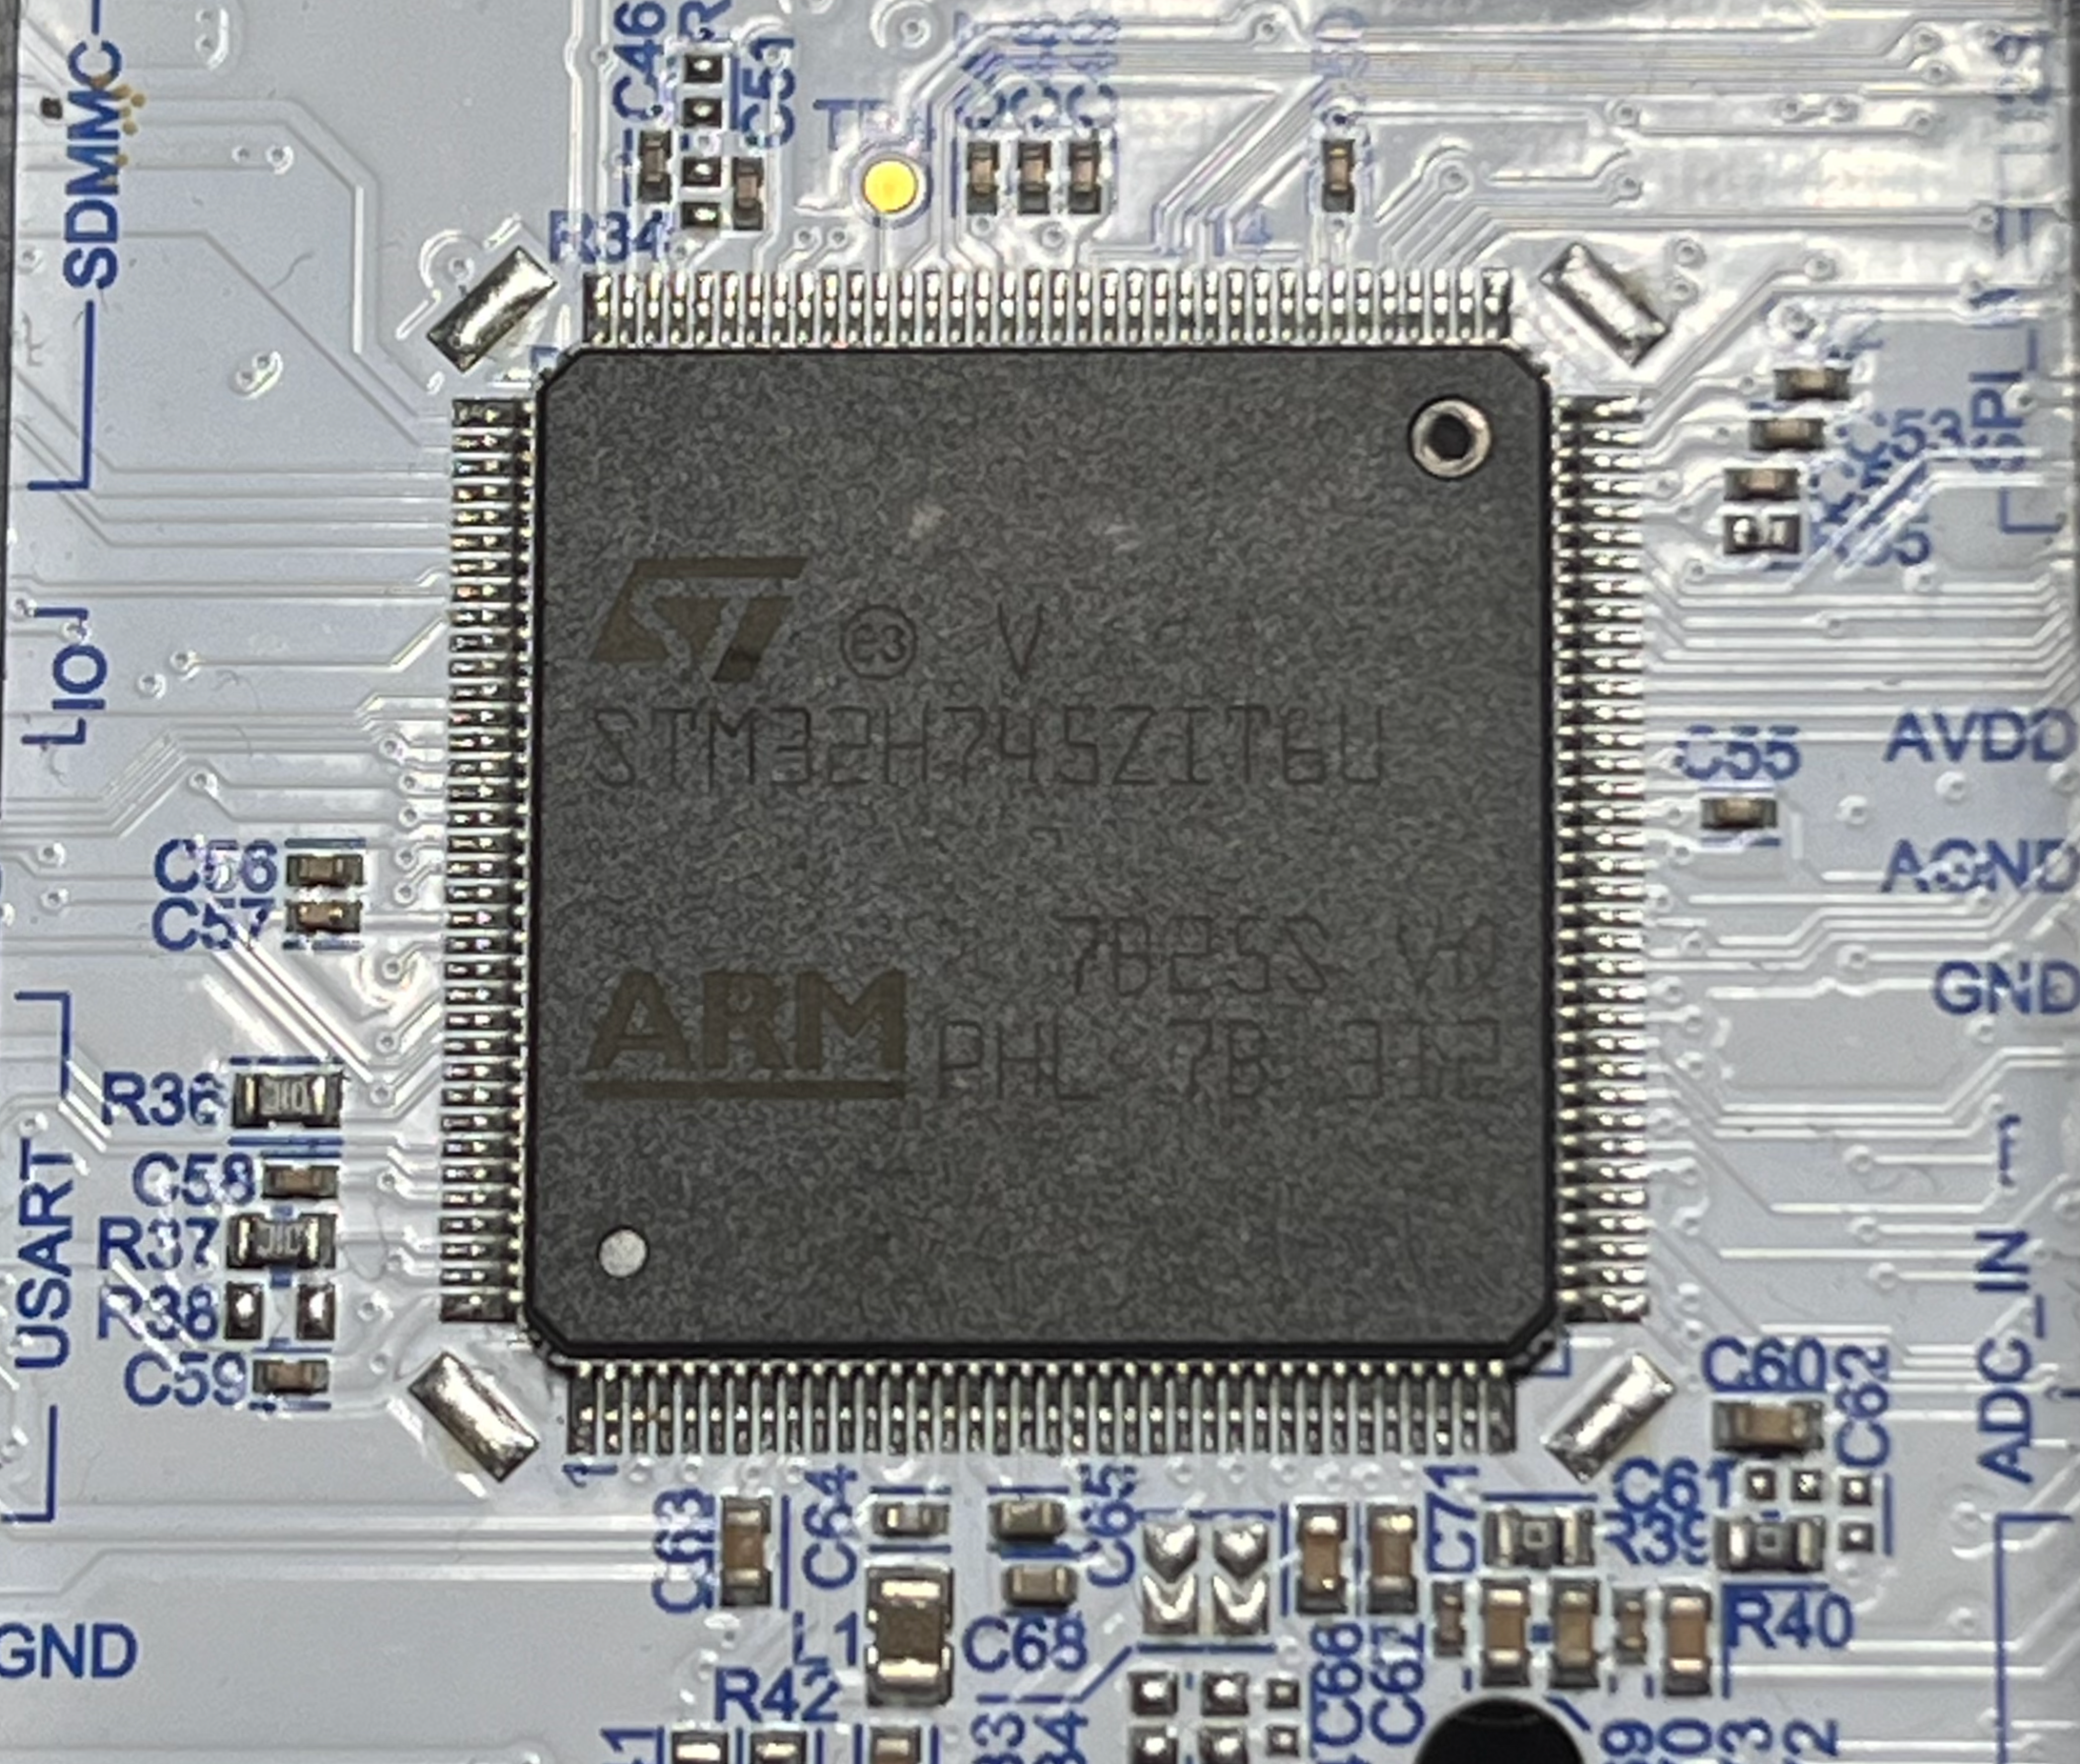
\includegraphics[width=0.5\textwidth]{chapters/Chapter2-HARDWARE/Figures/IMG2-STM32H745ZI-TQ6.png}
    \caption{\textcolor{black}{Il microcontrollore STM32H745ZI-TQ6}}
    \label{fig:etichetta}
\end{figure}
%%%%%%%%%%%%%%%%%%%%%%%%%%%%%%%%%%%%%%%%%%%%%%%%%%%%%%%%%%%%%%%%%%%%%%%%%%%%%%%%%%%%%%%%%%%%%%%%%%%%%%%%%%%%%%%%%%%%%%%%%%%%%%%%%%%%%%%%%%%

%%%%%%%%%%%%%%%%%%%%%%%%%%%%%%%%%%%%%%%%%%%%%%%%%%%%%%%%%%%%%%%%%%%%%%%%%%%%%%%%%%%%%%%%%%%%%%%%%%%%%%%%%%%%%%%%%%%%%%%%%%%%%%%%%%%%%%%%%%%%%%%%%%%%%%%%%%%%%%%%%%%%%%%%%%%%%%%%%%%%%%%%%%%%%%%%%%%%%%%%%%%%%%%%%%%%%%%%%%%%%%%%
%%%%%%%%%%%%%%%%%%%%%%%%%%%%%%%%%%%%%%%%%%%%%%%%%%%%%%%%%%%%%%%%%%%%%%%%%%%%%%%%%%%%%%%%%%%%%%%%%%%%%%%%%%%%%%%%%%%%%%%%%%%%%%%%%%%%%%%%%%%%%%%%%%%%%%%%%%%%%%%%%%%%%%%%%%%%%%%%%%%%%%%%%%%%%%%%%%%%%%%%%%%%%%%%%%%%%%%%%%%%%%%%

\subsection{{Caratteristiche della scheda NUCLEO-H745ZI-Q}}
La NUCLEO-H745ZI-Q è la scheda di sviluppo (\textit{development board}) che proietta all'esterno tutte le funzionalità del microcontrollore poco fa descritto.

\paragraph{ST-LINK/V3E}\mbox{}\\
L'ST-LINK/V3E è un'interfaccia hardware, gestita dal microcontrollore STM32F723, dedicata al collegamento tra elboratore esterno e microcontrollore. Il modulo permette di caricare il compilato \textit{firmware} sul microcontrollore direttamente dalla porta USB Micro-B collegata al sistema di elaborazione.
Il modulo, permette, inoltre, di eseguire il \textit{debug} in tempo reale del codice caricato sull'\textit{MCU}\textcolor{blue}{[A]}.\\
L'ST-LINK/V3E fornisce anche interfacce ausiliarie utili ai fini dello sviluppo.\\
A seguire un breve elenco esplicativo di queste funzionalità aggiuntive:
\begin{itemize}
    \item VCP (\textit{Virtual COM Port}): lo ST-LINK crea una porta seriale virtuale via USB, in tal modo è possibile collegarsi al microcontrollore come se fosse collegato via UART classica.
    \item MSC (\textit{Mass Storage}): la scheda di sviluppo appare al sistema di elaborazione come una memoria esterna.
\end{itemize}

\paragraph{Alimentazione}\mbox{}\\
La scheda di sviluppo offre diversi approcci per l'alimentazione: 
\begin{itemize}
    \item Alimentazione via USB Micro-B ST-LINK a 5V.
    \item Alimentazione via Jack esterno da 7-12V.
    \item Alimentazione tramite \textit{pin Vin} esterno a 3.3V.
\end{itemize}
Nonostante la presenza di diversi approci di alimentazione e i differenti voltaggi, la tensione di alimentazione del microcontrollore è 3.3V \textcolor{red}{Rev}, ottenuta attraverso regolatori interni.

\paragraph{Formato fisico}\mbox{}\\
La scheda di sviluppo in esame appartiene alla famiglia \textbf{Nucleo-144} di STMicroelectronics e, dunque, mette a disposizione 2 connettori \textbf{\textit{Morpho}} che espongono i 144 \textit{pin} del microcontrollore. Il sistema di espansione poco fa citato viene chiamato ST Zio.\\
La NUCLEO-H745ZI-Q offre, inoltre, la compatibilità hardware e pinout con gli \textit{Shield Arduino Uno R3}.\\
\textcolor{red}{\Large{DESCRIVI QUALI PERIFEIRCHE HAI UTILIZZATO PER IL PROGETTO E PERCHé }}

%%%%%%%%%%%%%%%%%%%%%%%%%%%%%%%%%%%%%%%%%%%%%%%%%%%%%%%%%%%%%%%%%%%%%%%%%%%%%%%%%%%%%%%%%%%%%%%%%%%%%%%%%%%%%%%%%%%%%%%%%%%%%%%%%%%%%%%%%%%
\begin{figure}[htbp]
    \centering
    \includegraphics[width=0.6\textwidth]{chapters/Chapter2-HARDWARE/Figures/IMG1-FotoDaSopraScheda.png}
    \caption{\textcolor{black}{La scheda di sviluppo  NUCLEO-H745ZI-Q}}
    \label{fig:etichetta}
\end{figure}
%%%%%%%%%%%%%%%%%%%%%%%%%%%%%%%%%%%%%%%%%%%%%%%%%%%%%%%%%%%%%%%%%%%%%%%%%%%%%%%%%%%%%%%%%%%%%%%%%%%%%%%%%%%%%%%%%%%%%%%%%%%%%%%%%%%%%%%%%%%
